\documentclass[12pt,a4paper]{scrartcl}
\usepackage[utf8]{inputenc}
\usepackage[english,russian]{babel}
\usepackage{indentfirst}
\usepackage{misccorr}
\usepackage{graphicx}
\usepackage{amsmath}
\usepackage{multirow}
\usepackage{pgfplots}
\usepackage{parskip}
\usepackage[top=1cm, bottom=1cm, left=1cm, right=1cm]{geometry}
\pgfplotsset{compat=1.9}

\begin{document}
	\graphicspath{{py/}}
	
	\newcommand{\ms}{\mathstrut}
	\newcommand{\msp}{\hspace{0.5cm}}
	\newcommand{\al}{\alpha}
	\newcommand{\dg}{^\circ}
	\newcommand{\dif}{\mathrm{d}}
	\newcommand{\qd}[2]{^{\frac{#1}{#2}}}
	\newcommand{\qdm}[2]{^{-\frac{#1}{#2}}}
	\newcommand{\lm}[2]{\underset{#1 \rightarrow #2}{\lim}}
	\newcommand{\sfrac}[2]{\dfrac{\strut #1}{\strut #2}}
	\newcommand{\equal}[1]{\overset{(#1)}{=}}
	\newcommand{\linevdots}{\ \raisebox{-.08\height}{\vdots}\ }
	\newcommand{\linecvdots}{\ \raisebox{-.08\height}{\vdots}\hspace{-0.13cm}\raisebox{.15\height}{\cancel{\phantom{a}}\hspace{0.06cm}}}
	\newcommand{\combox}[1]{\ms \msp \msp \begin{minipage}{0.95\linewidth}
			#1
	\end{minipage}}
	
	\newtheorem{pr}{Задача}
	\newtheorem{ex}{Пример}
	\newtheorem{dfn}{Def}
	\newtheorem{theorem}{Th}
	
	\newenvironment{slv}{\ms \msp \textit{Решение:}}{}
	\newenvironment{proof}{\ms \msp \textit{Доказательство: }}{\hfill $\square$}
	
	\begin{titlepage}
		
		\vspace*{\fill}
		
		\begin{center}
			
\includegraphics[scale=0.8]{MIPT.png}
			\\[0.7cm]\Huge Московский Физико-Технический Институт\\(национальный исследовательский университет)
			\\[2cm]\LARGE Отчет по эксперименту
			\\[0.5cm]\noindent\rule{\textwidth}{1pt}
			\\\Huge\textbf{Спектральный анализ электрических сигналов}
			\\[-0.5cm]\noindent\rule{\textwidth}{1pt}
		\end{center}
		
		\begin{flushleft}
			\textit{Работа №3.6.1; дата: 07.10.22}\hfill\textit{Семестр: 3}
		\end{flushleft}
		
		\vspace*{\fill}
		
		\begin{flushleft}
			Выполнил: \hspace{\fill} Группа:
			\\Кошелев Александр \hspace{\fill} Б05-105
		\end{flushleft}
	\end{titlepage}
	
	%Страница 2
	
	\begin{flushleft}
		\footnotesize{Спектральный анализ электрических сигналов} \hspace{\fill} \footnotesize{2}
		\\[-0.3cm]\noindent\rule{\textwidth}{0.3pt}
	\end{flushleft}
	
	\section{Аннотация}
	
	\textbf{Цель работы: }
	
	Изучить спектральный состав периодических электрических сигналов.
	
	\textbf{Схема установки:}
	\begin{center}
		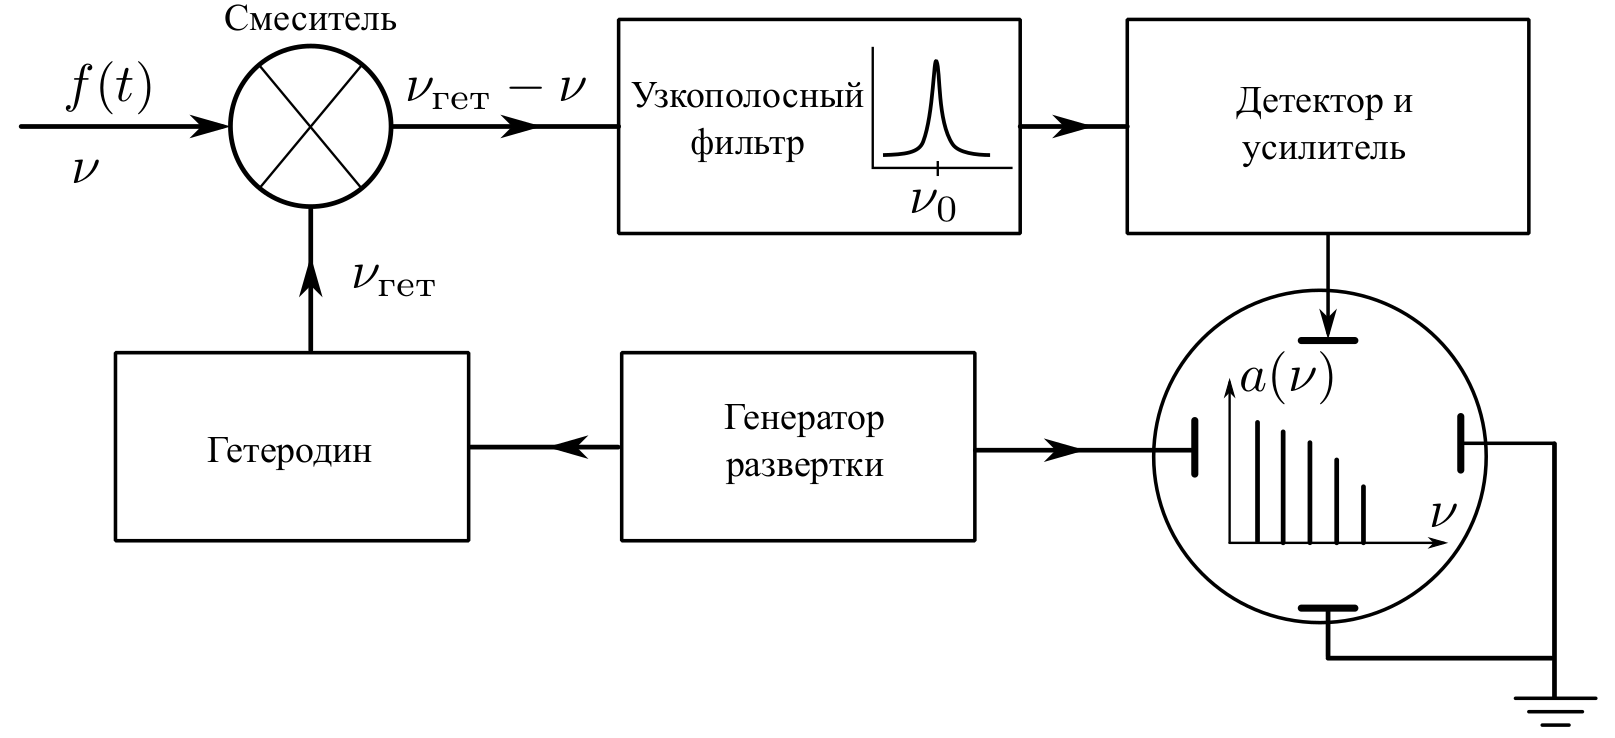
\includegraphics[scale=0.25]{PIC_1.png}
		\\\textbf{Рис. 1:} Схема установки
	\end{center}	
		
	Как правило, для фильтрации сигнала применяется следующая схема. Исследуемый сигнал $f(t)$ и синусоидальный сигнал от вспомогательного генератора, называемого в таких системах \textit{гетеродином}, подаются на вход \textit{смесителя}. Смеситель — элемент, преобразующий колебания с частотами $\nu_1$ и $\nu_2$ в колебания на комбинированных частотах: $\nu_1 + \nu_2$ и $\nu_1 - \nu_2$. «Разностный» сигнал смесителя поступает на фильтр -- высокодобротный колебательный контур, настроенный на некоторую фиксированную резонансную частоту $\nu_0$ . Таким образом, если $f(t)$ содержит гармонику $\nu = \nu_{\text{гет}} - \nu_0$ ($\nu_{\text{гет}}$ -- частота гетеродина), она будет	усилена, а отклик будет пропорционален её амплитуде. Отметим, что смешение частот исследуемого сигнала и частоты гетеродина лежит в основе большинства современных радиоприёмных устройств -- супергетеродинов.
	
	В спектральном анализаторе частота гетеродина пропорциональна напряжению, подаваемому на развёртку по оси $X$ встроенного в анализатор осциллографа. Выходной сигнал подаётся на канал $Y$. На экране анализатора возникает, таким образом, график, изображающий зависимость амплитуды гармоник исходного сигнала от частоты, то есть его спектр (заметим, что информация о фазах гармоник при этом теряется).
	
	В последнее время повсеместное распространение получила цифровая обработка сигналов. Спектральный состав оцифрованного сигнала может быть найден численно. Существуют алгоритмы (быстрое преобразование Фурье, FFT), позволяющие проводить вычисления коэффициентов Фурье в реальном времени для сигналов относительно высокой	частоты (до 200 МГц). Гетеродинные схемы по-прежнему применяются для анализа спектров сверхвысоких частот, приближающихся к тактовой частоте современных интегральных схем ($\gtrsim$1 ГГц).
		
	\textbf{В работе используются:}
	
	Генератор сигналов специальной формы, электронный осциллограф с выводом информации на компьютер, компьютер с ПО для анализа поступающего сигнала.
	
	\newpage
	
	%Страница 3
	
	\begin{flushleft}
		\footnotesize{Спектральный анализ электрических сигналов} \hspace{\fill} \footnotesize{3}
		\\[-0.3cm]\noindent\rule{\textwidth}{0.3pt}
	\end{flushleft}
	
	\section{Теоретические сведения}
	
	В работе изучается спектральный состав периодических электрических сигналов различной формы: последовательности прямоугольных импульсов, последовательности цугов и амплитудно-модулированных гармонических колебаний. Спектры этих сигналов наблюдаются с помощью анализатора спектра и сравниваются c рассчитанными теоретически.
	
	Периодическая функция может быть представлена в виде бесконечного ряда гармонических функций — ряда Фурье:
	
	$$f(t) = \sum_{n = -\infty}^{+\infty} c_n\exp(i n \omega_o t) \ \ \ \ \ \ \ \ f(t) = \sum_{n = 0}^{+\infty} a_n \cos (n \omega_0 t + \varphi_n)$$
	
	Здесь $\omega_0 = \frac{2\pi}{T}$ , где $T$ — период функции $f(t)$. Коэффициенты {$c_n$} могут быть найдены по формуле:
	
	$$c_n = \sfrac{1}{T} \int_{0}^{T} f(t) \exp(-i n \omega_0 t)\, \dif t$$
	
	Наборы коэффициентов разложения в комплексной \{$c_n$\} и действительной \{$a_n, \varphi_n$\} формах связаны соотношением:
	
	$$a_n = 2|c_n| \ \ \ \ \ \ \ \ \varphi_n = \arg (c_n)$$
	
	В качестве простейшего спектрального анализатора можно использовать высокодобротный	колебательный контур с подстраиваемой ёмкостью или индуктивностью:
	
	\begin{center}
		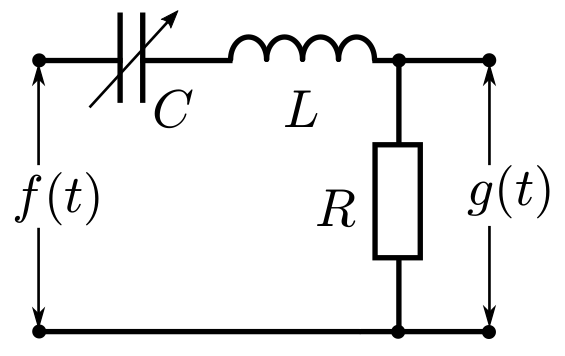
\includegraphics[scale=0.25]{PIC_2.png}
		\\\textbf{Рис. 2:} Колебательный контур как узкополостный фильтр
	\end{center}

	Такой контур усиливает те гармоники входного сигнала $f(t)$, частота которых близка к резонансной $\nu_0 = 2\pi / \sqrt{LC}$ и практически не реагирует на частоты, далёкие от $\nu_0$.
	
	С точки зрения преобразования гармоник колебательный контур является узкополосным \textit{фильтром} с шириной полосы пропускания порядка $\Delta \nu \sim \frac{\nu_0}{Q}$ где $Q = \sfrac{1}{R} \sqrt{\frac{L}{C}} \gg 1$ — его добротность. Амплитуда колебаний в контуре пропорциональна амплитуде $|c(\nu_0)|$ гармоники в спектре функции $f(t)$, частота которой совпадает с $\nu_0$. Таким образом, меняя резонансную частоту контура, можно «просканировать» весь спектр входного сигнала.
	
	У описанной выше схемы есть существенный недостаток: при изменении $L$ или $C$ меняется также и добротность, а значит, и ширина полосы пропускания. Кроме того, проще изготовить высокодобротный контур с фиксированными параметрами, нежели с настраиваемой частотой. В связи с этим, как правило, для фильтрации сигнала применяется применяется схема нашей установки.
	
	\newpage
	
	%Страница 4
	
	\begin{flushleft}
		\footnotesize{Спектральный анализ электрических сигналов} \hspace{\fill} \footnotesize{4}
		\\[-0.3cm]\noindent\rule{\textwidth}{0.3pt}
	\end{flushleft}
	
	\section{Проведение эксперимента}
	
	\paragraph{Исследование спектра периодической последовательности прямоугольных импульсов} \hfill
	
	\paragraph{Качественное исследование} \hfill
	
	Вначале качественно пронаблюдаем за получаемыми спектрами:
	
	\begin{figure}[h]
		\begin{minipage}{0.5\linewidth}
			\begin{center}
				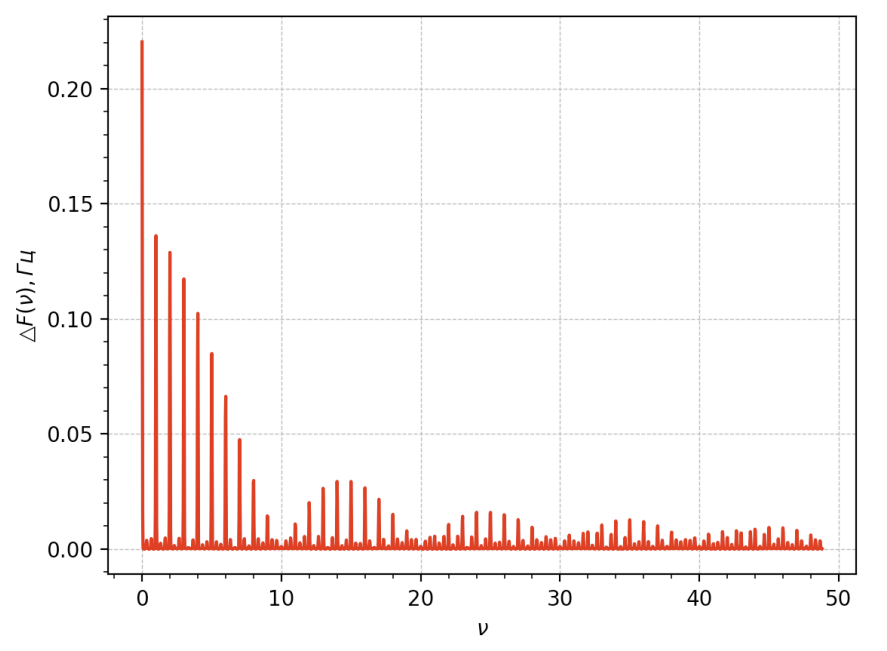
\includegraphics[scale=0.247]{PIC_3.png}
				\\\textbf{Рис. 3:} Спектр при $\nu = 1$ kHz, $\tau = 50$ $\mu$s
			\end{center}
		\end{minipage}
		\begin{minipage}{0.5\linewidth}
			\begin{center}
				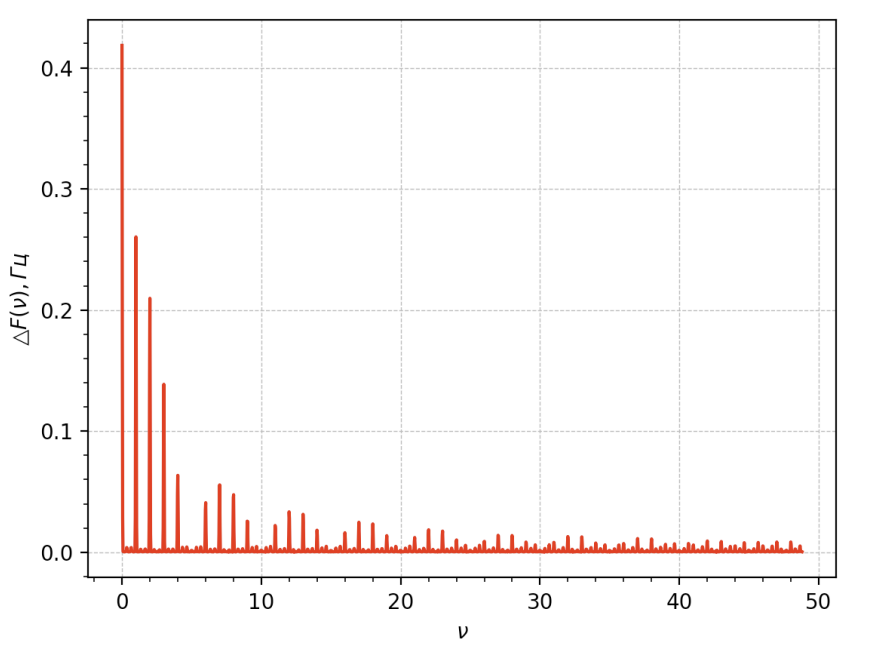
\includegraphics[scale=0.25]{PIC_4.png}
				\\\textbf{Рис. 4:} Спектр при $\nu = 1$ kHz, $\tau = 100$ $\mu$s
			\end{center}
		\end{minipage}
	\end{figure}

	\begin{center}
		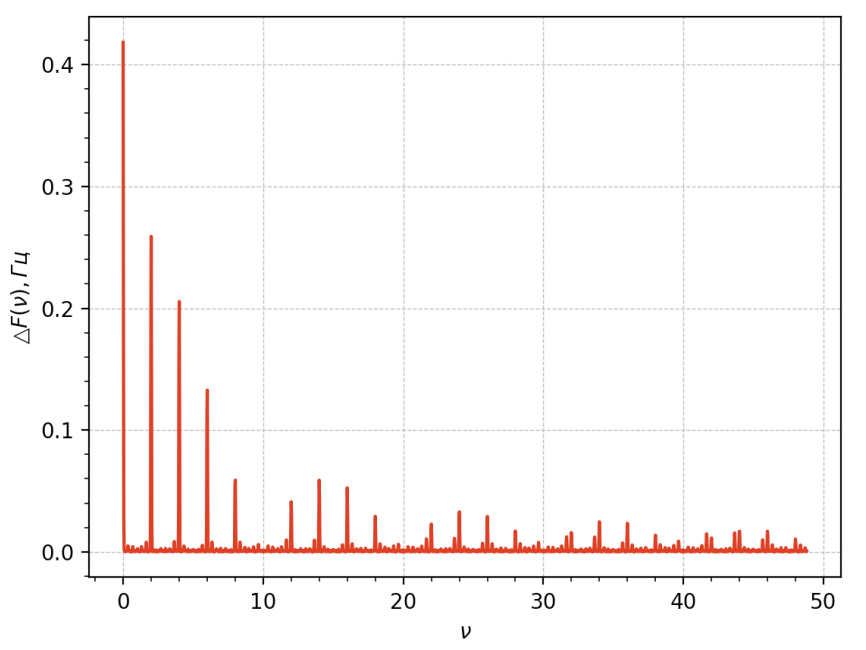
\includegraphics[scale=0.25]{PIC_5.png}
		\\\textbf{Рис. 5:} Спектр при $\nu = 2$ kHz, $\tau = 50$ $\mu$s
	\end{center}

	Из вида данных спектров можно убедиться в справедливости основных масштабов спектра:
	
	$$\Delta \nu_\tau = \sfrac{1}{\tau} \ \ \ \ \ \ \ \ \Delta \nu_T = \sfrac{1}{T} = \nu_{\text{ген}} \ \ \ \ \ \ \ \ \Delta \nu_0 = \sfrac{1}{t_0}$$
	
	\paragraph{Количественное исследование} \hfill
	
	Зафиксируем частоту генерации меандра равной 1 kHz. Снимем зависимость $\Delta \nu (1/\tau)$:
	
	\begin{center}
		\begin{tabular}{|c|c|c|c|c|c|c|c|c|c|}
			\hline
			$\tau$, $\mu$s & 40 & 60 & 80 & 100 & 120 & 140 & 160 & 180 & 200
			\\\hline
			$\Delta \nu \pm 0.5$, kHz & 25.0 & 17.0 & 13.0 & 10.0 & 8.0 & 7.0 & 6.0 & 5.5 & 5.0
			\\\hline
		\end{tabular}
		\\\textbf{Табл. 1:} Зависимость $\nu (\tau)$
	\end{center}
	
	По полученным данным построим график зависимости $\nu(1/\tau)$.
	
	\newpage
	
	%Страница 5
	
	\begin{flushleft}
		\footnotesize{Спектральный анализ электрических сигналов} \hspace{\fill} \footnotesize{5}
		\\[-0.3cm]\noindent\rule{\textwidth}{0.3pt}
	\end{flushleft}
	
	\begin{center}
		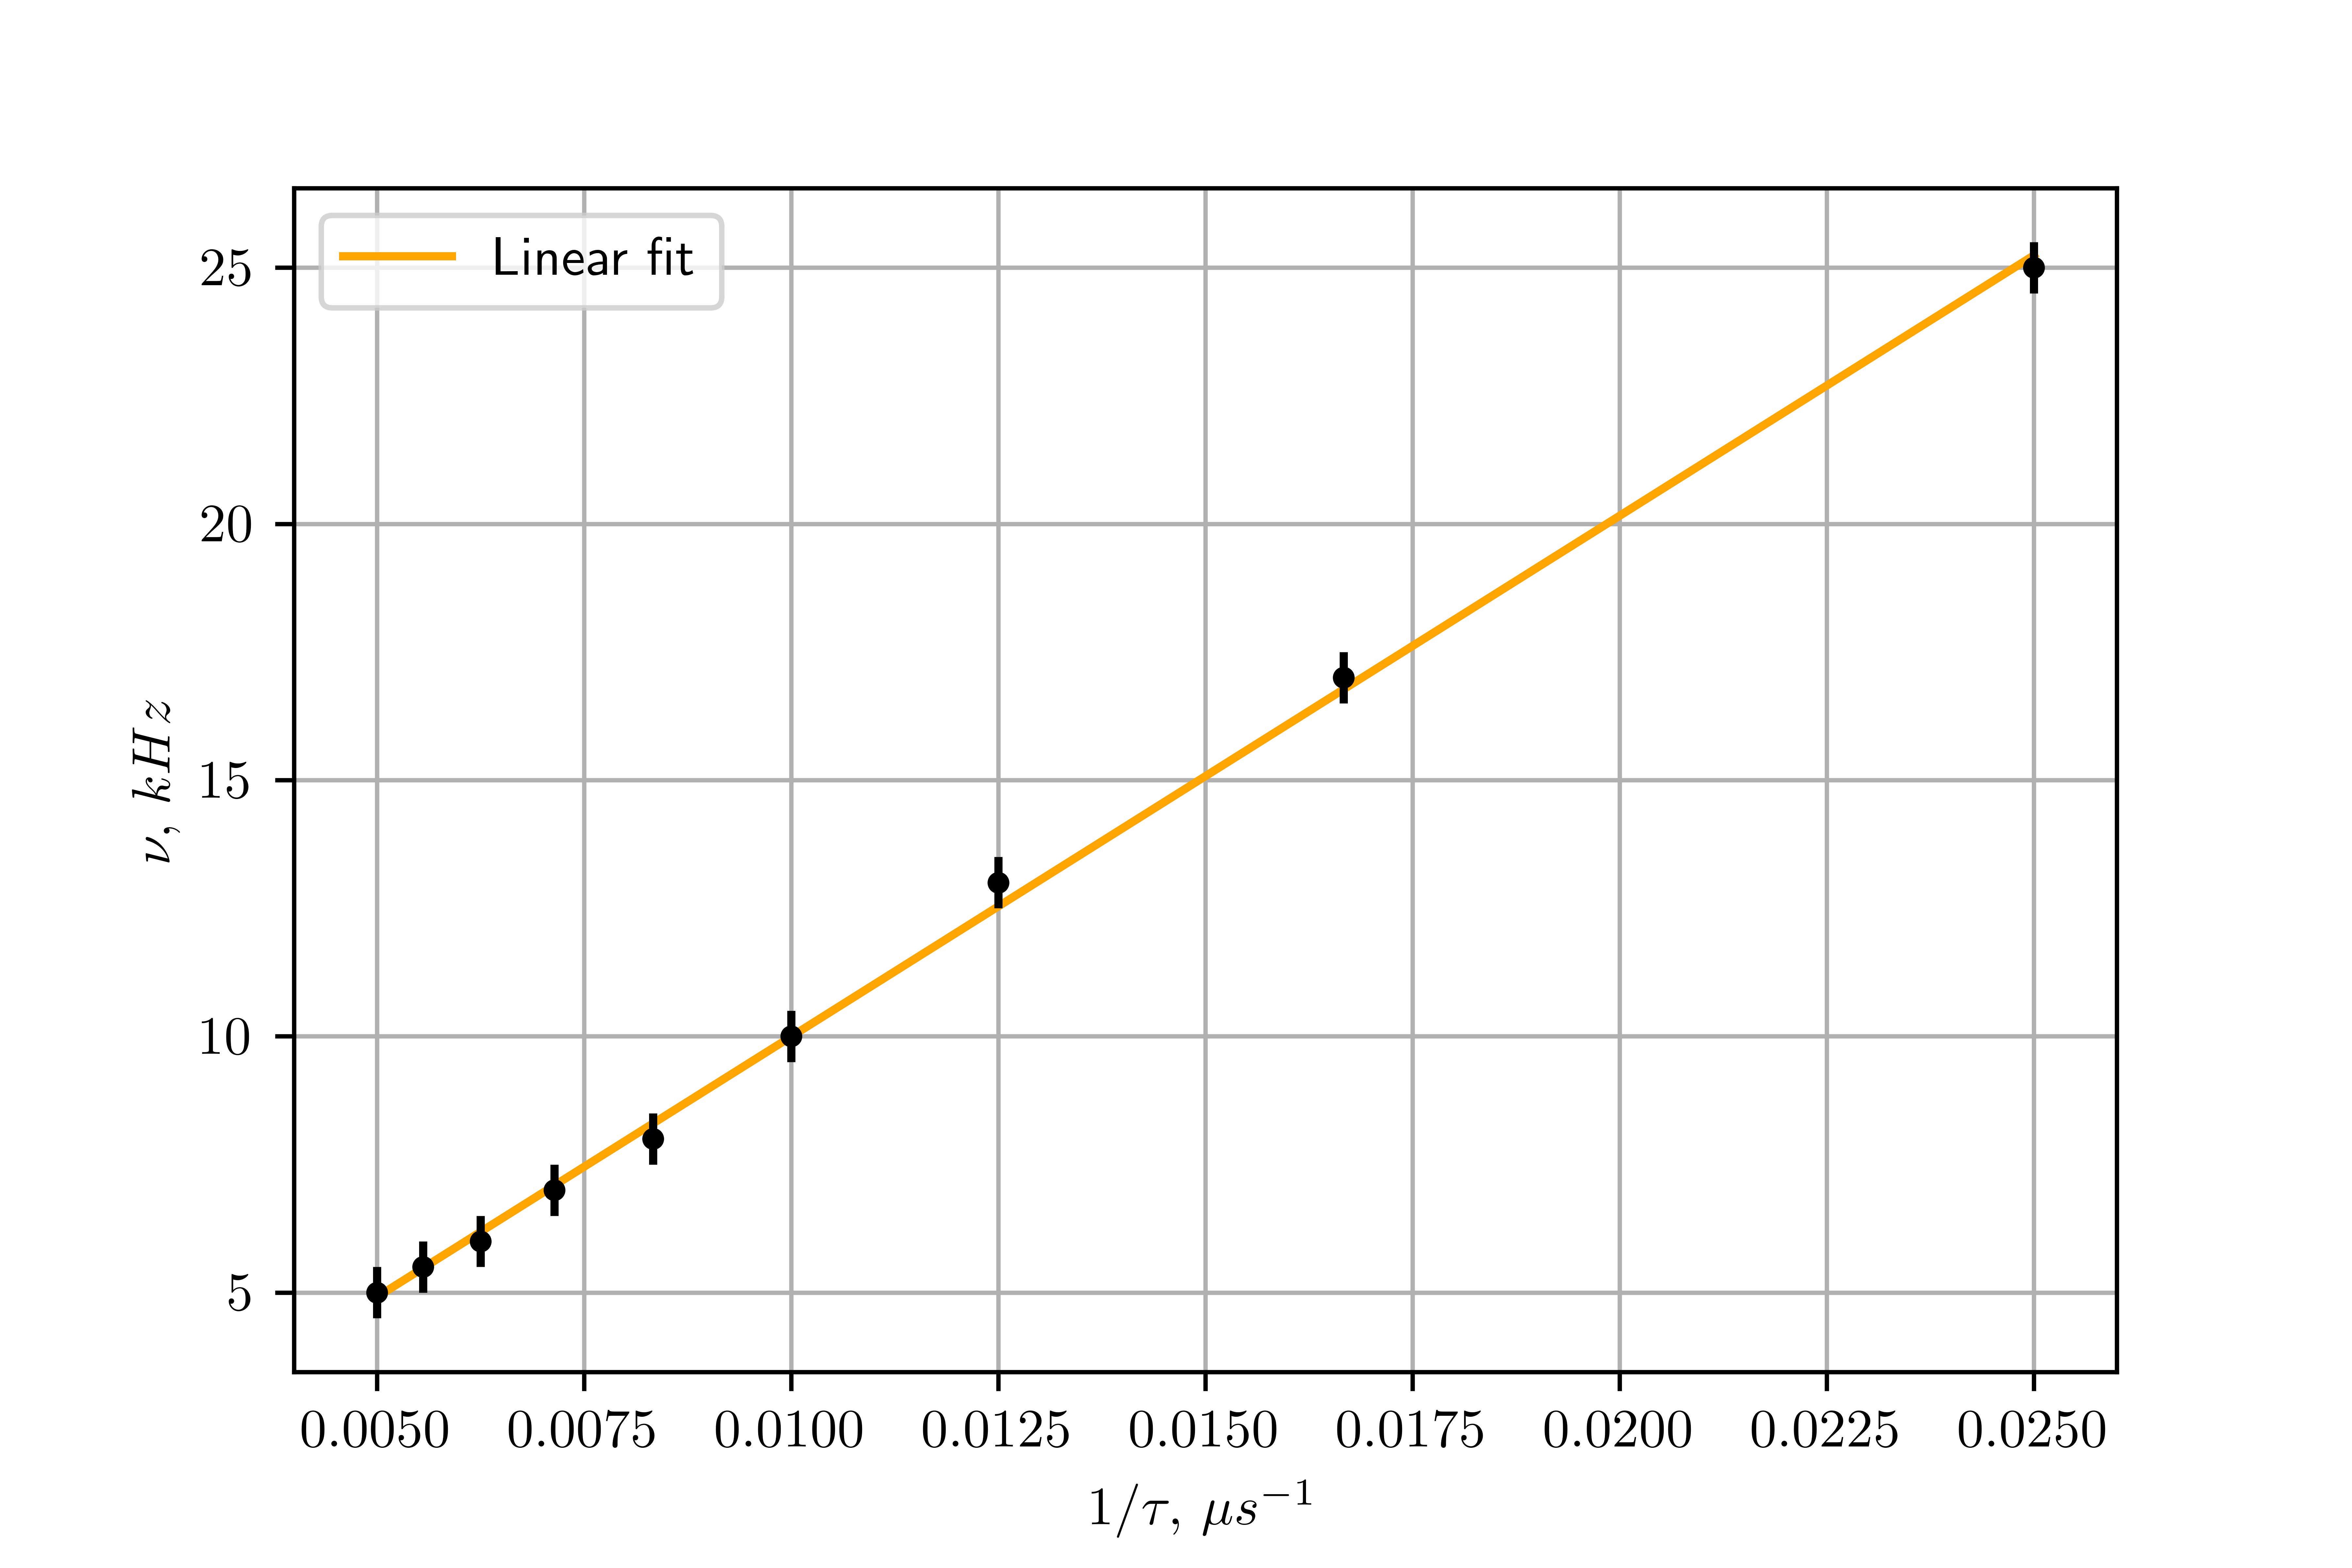
\includegraphics[scale=1]{PIC_6.png}
		\\\textbf{Рис. 6:} График зависимости $\nu(1/\tau)$
	\end{center}
	
 	Из графика видно, что точки хорошо ложатся на прямую. Представив прмяую в виде $\nu = k(1/\tau) + b$, получаем методом линейной аппроксимации $k = (1016 \pm 13)\, \text{kHz} \cdot \mu s$, $b = (-0.16 \pm 0.17)$. При этом величина $b$ лежит в рамках стандартного отклонения, что свидетельствует о справедливости соотношения неопределенностей $\Delta \nu \sim 1/\tau$.
	
	\paragraph{Исследование спектра периодической последовательности цугов} \hfill
	
	\paragraph{Качественное исследование} \hfill
	
	Вначале качественно пронаблюдаем за получаемыми спектрами в зависимости от длины цуга:
	
	\begin{figure}[h]
		\begin{minipage}{0.5\linewidth}
			\begin{center}
				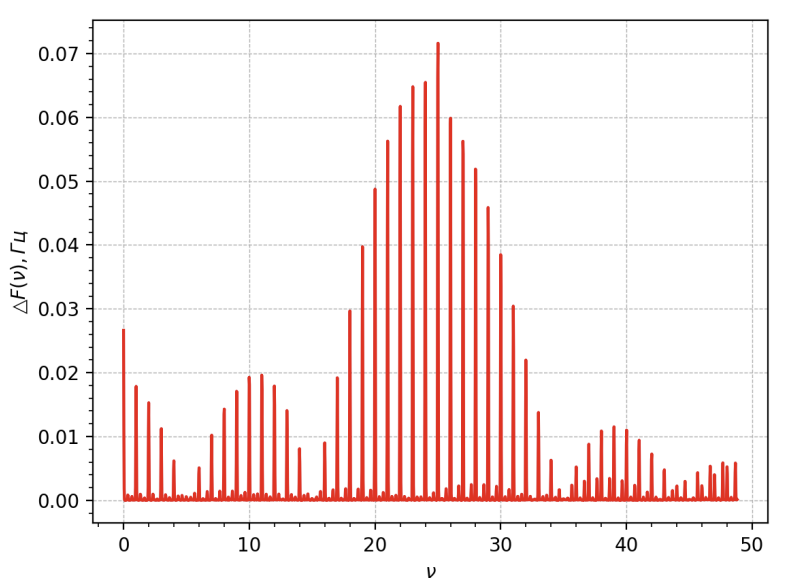
\includegraphics[scale=0.247]{PIC_7.png}
				\\\textbf{Рис. 7:} Спектр при $\nu_0 = 25$ kHz, $\tau = 50$ $\mu$s
			\end{center}
		\end{minipage}
		\begin{minipage}{0.5\linewidth}
			\begin{center}
				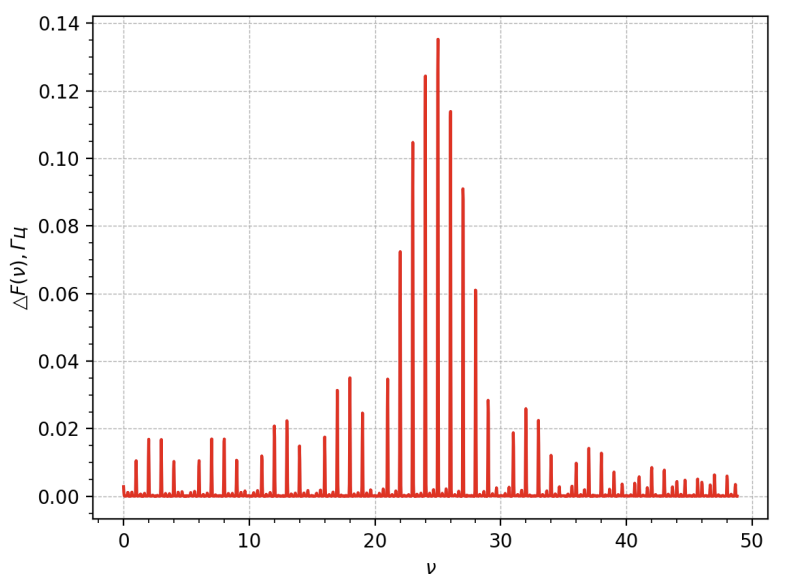
\includegraphics[scale=0.25]{PIC_8.png}
				\\\textbf{Рис. 8:} Спектр при $\nu_0 = 25$ kHz, $\tau = 100$ $\mu$s
			\end{center}
		\end{minipage}
	\end{figure}
	
	Главный пик спектрограммы попадает своим центром на несущую частоту. Можно при этом пронаблюдать эффект, аналогичный случаю меандра: уменьшение в два раза ширины пиков при увеличении длины импульса.
	
	Теперь попробуем изменять несущую частоту при постоянной длине импульса.
	
	
	\newpage
	
	%Страница 6
	
	\begin{flushleft}
		\footnotesize{Спектральный анализ электрических сигналов} \hspace{\fill} \footnotesize{6}
		\\[-0.3cm]\noindent\rule{\textwidth}{0.3pt}
	\end{flushleft}
	
	\begin{figure}[h]
		\begin{minipage}{0.5\linewidth}
			\begin{center}
				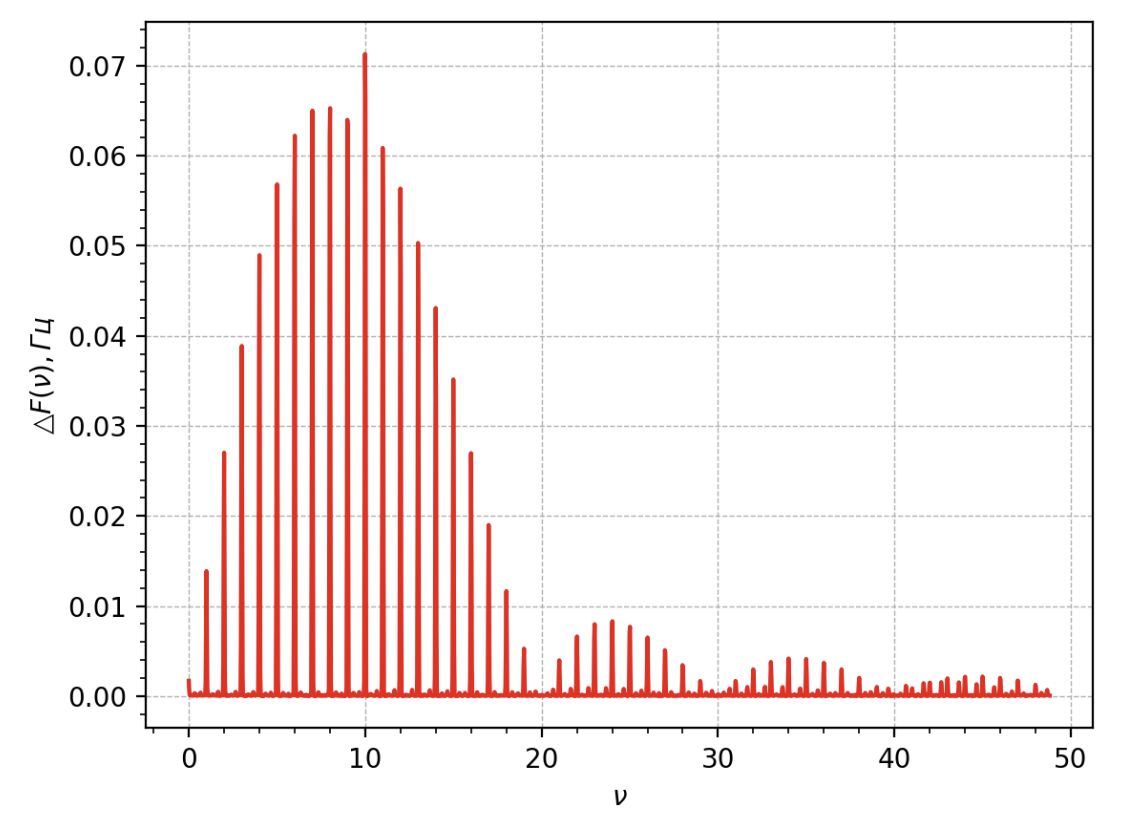
\includegraphics[scale=0.18]{PIC_9.png}
				\\\textbf{Рис. 9:} Спектр $\nu_0 = 10$ kHz, $\tau = 50$ $\mu$s
			\end{center}
		\end{minipage}
		\begin{minipage}{0.5\linewidth}
			\begin{center}
				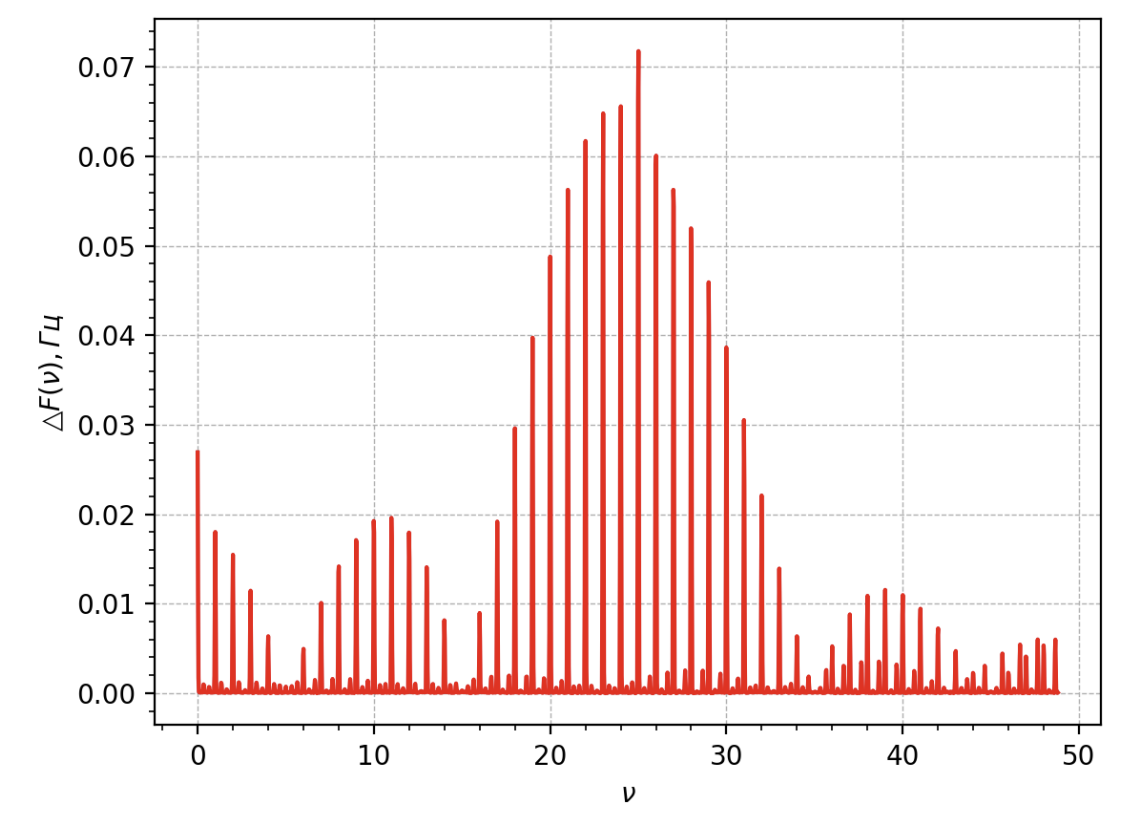
\includegraphics[scale=0.18]{PIC_10.png}
				\\\textbf{Рис. 10:} Спектр $\nu_0 = 25$ kHz, $\tau = 50$ $\mu$s
			\end{center}
		\end{minipage}
	\end{figure}

	\begin{center}
		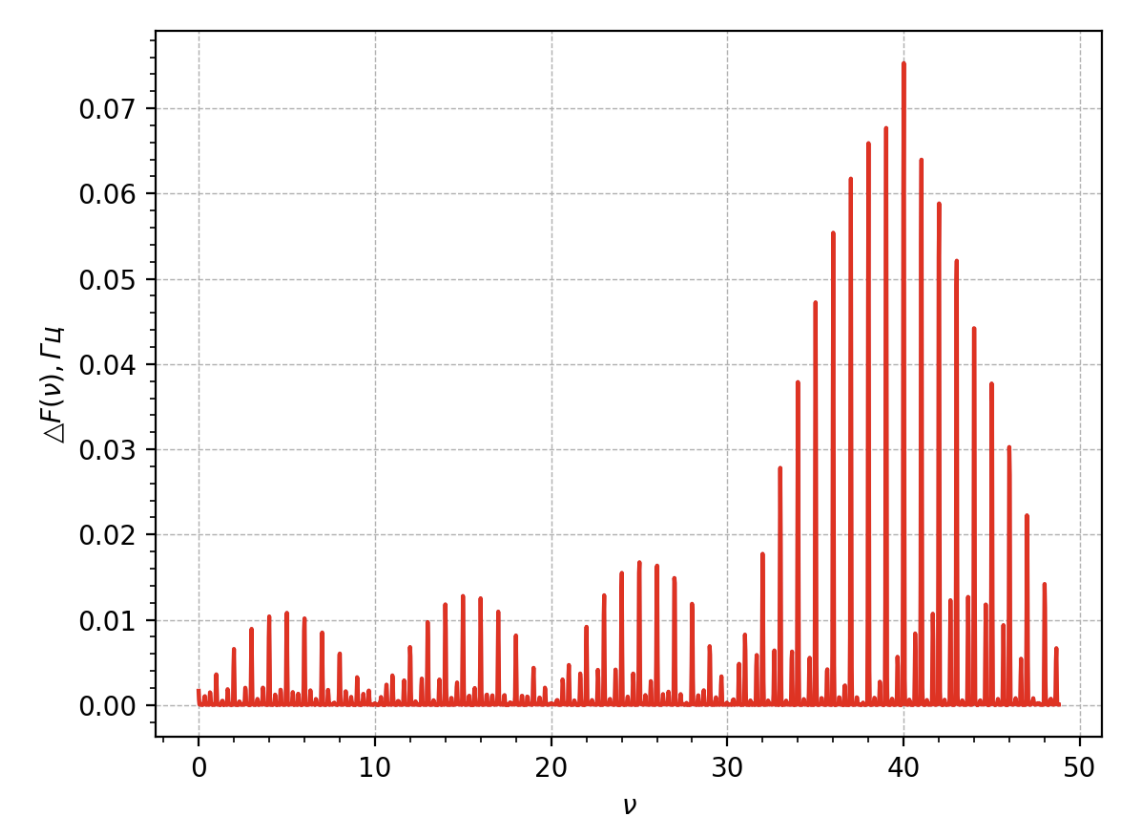
\includegraphics[scale=0.18]{PIC_11.png}
		\\\textbf{Рис. 11:} Спектр $\nu_0 = 40$ kHz, $\tau = 50$ $\mu$s
	\end{center}
	
	При смещении несущей частоты при постоянной длительности импульса не изменяется ширина пиков, но центр главного пика следует за частотой.
	
	\paragraph{Количественное исследование} \hfill
	
	Зафиксируем длину цуга равной $\tau = 50$ $\mu$s. Снимем зависимость $\delta \nu (1/T) = \delta \nu (\nu_0)$:
	
	\begin{center}
		\begin{tabular}{|c|c|c|c|c|c|}
			\hline
			$\nu_0$, kHz & 0.5 & 1 & 2 & 4 & 5
			\\\hline
			$\delta \nu$, kHz & 0.5 & 1.0 & 2.0 & 4.0 & 5.0
			\\\hline
		\end{tabular}
		\\\textbf{Табл. 2:} Зависимость $\delta \nu (1/T)$
	\end{center}
	
	По полученным данным построим график зависимости $\delta\nu(1/T)$.
	
		\begin{center}
		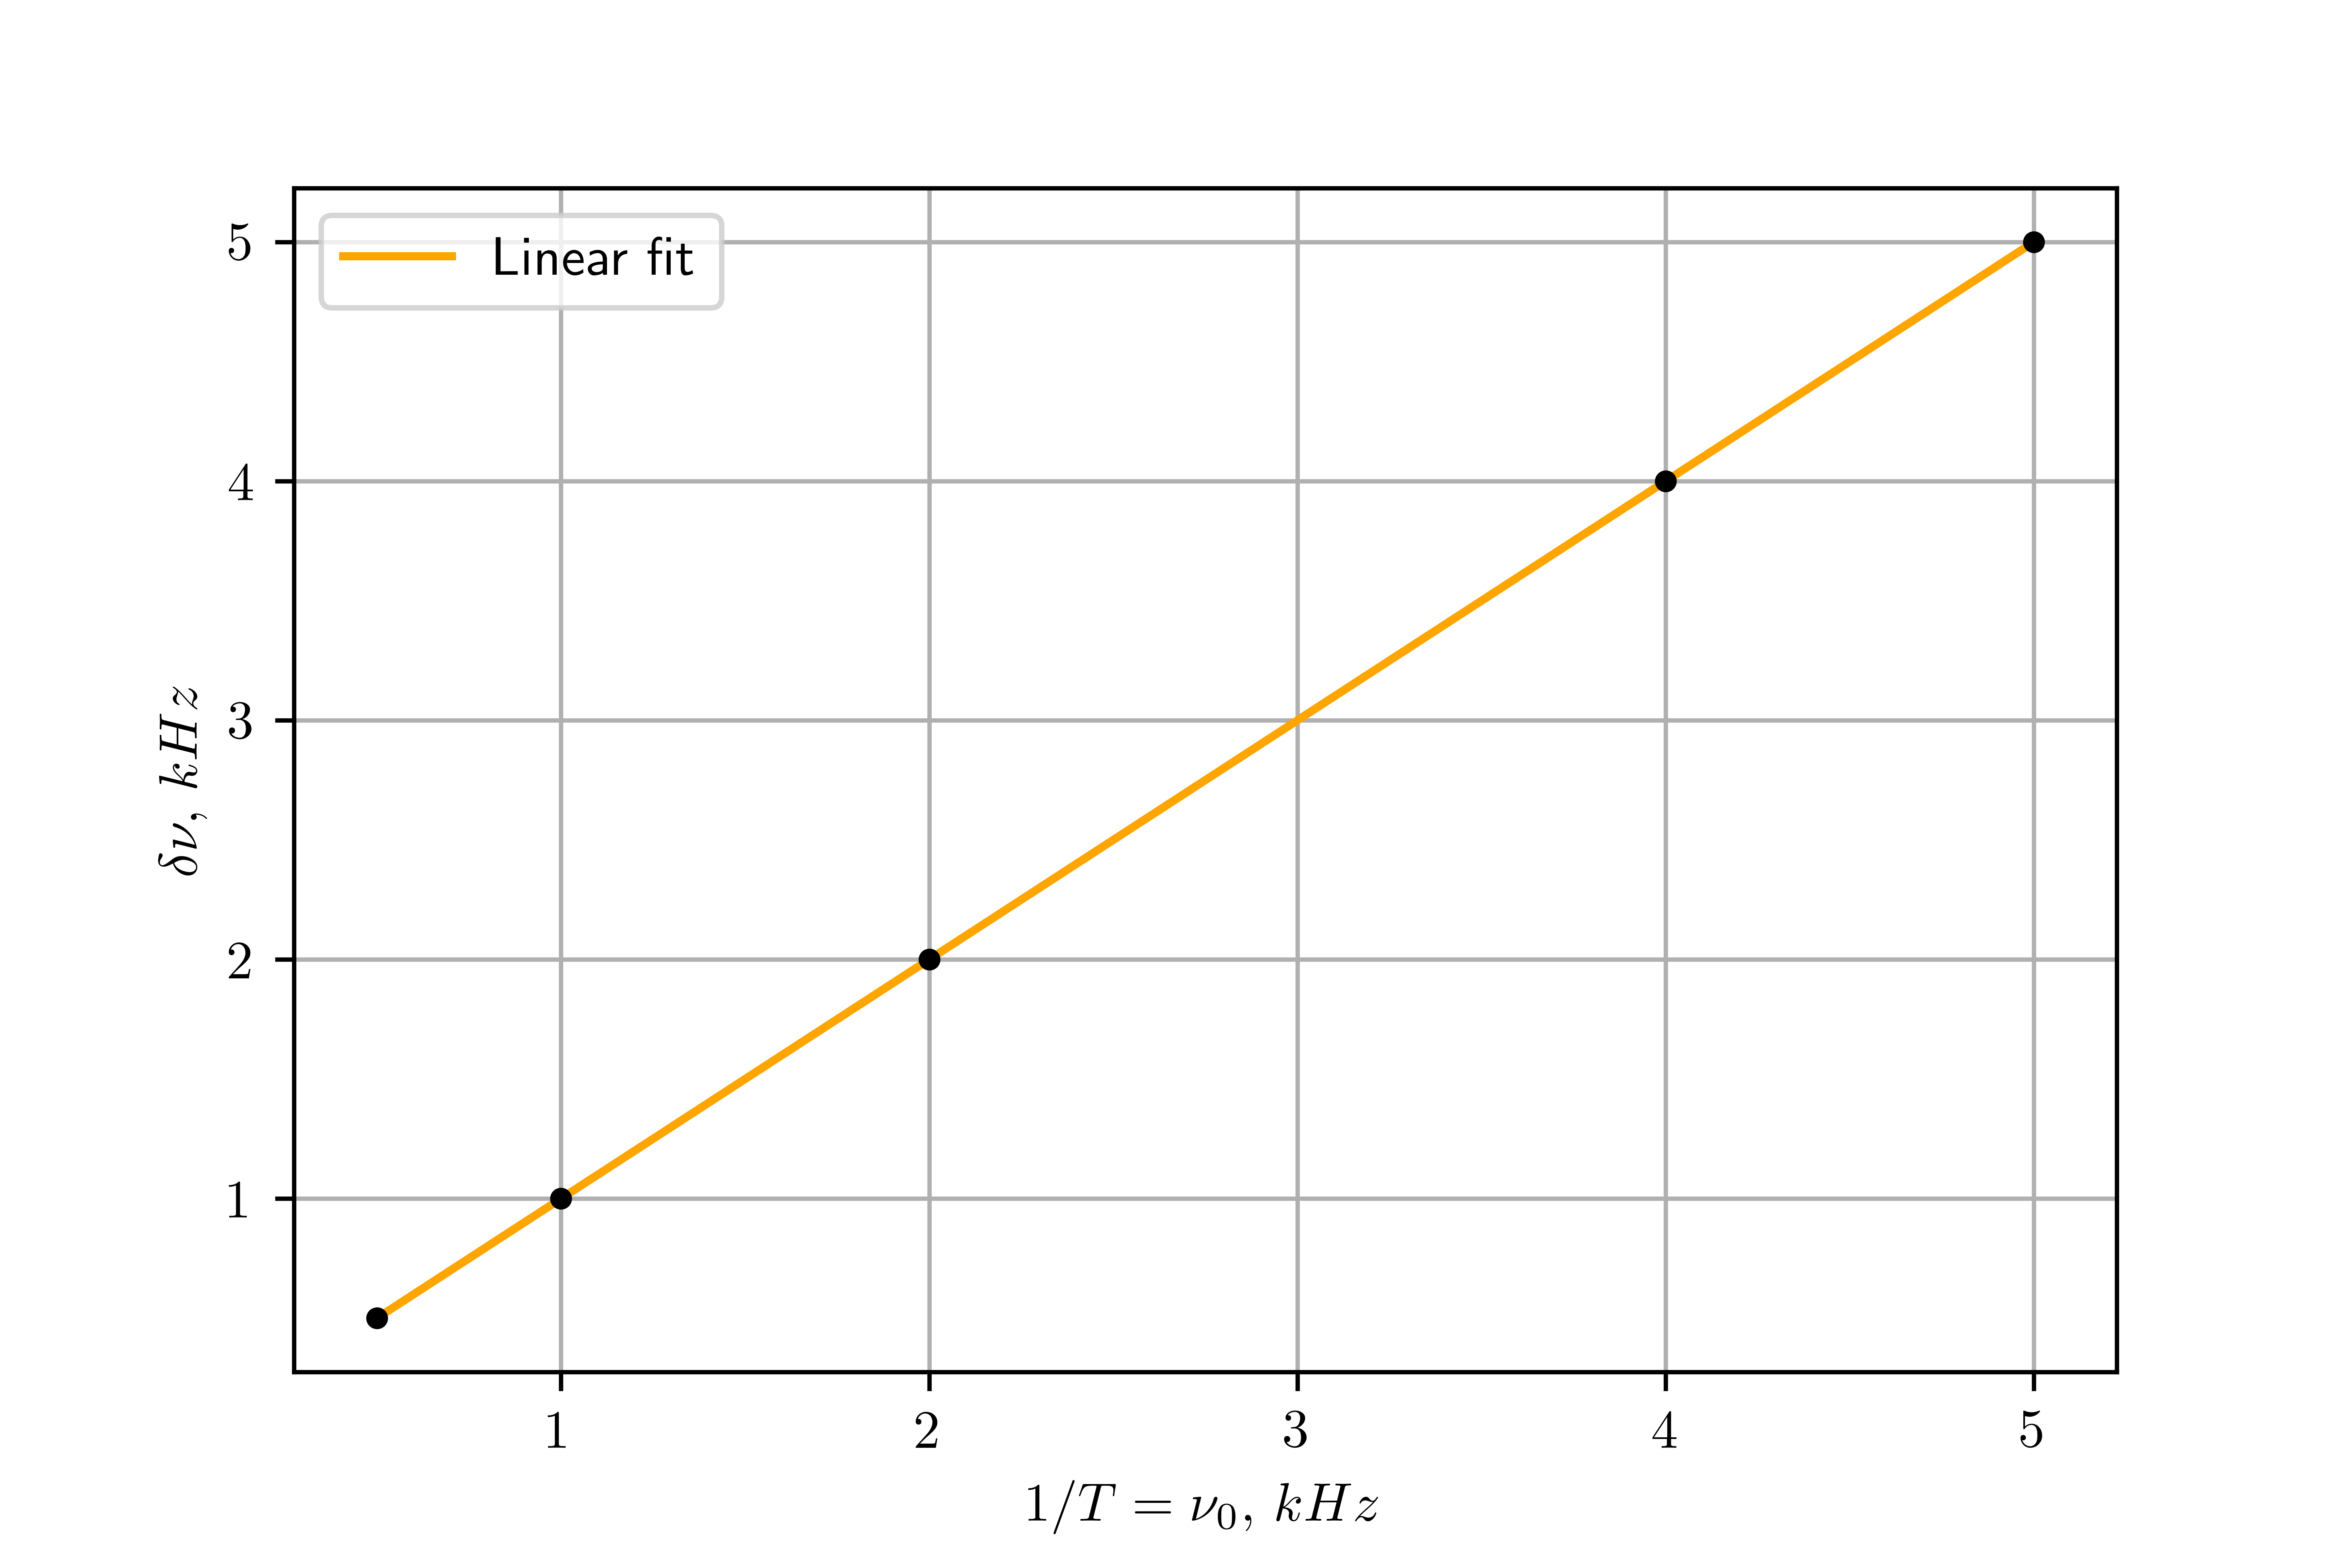
\includegraphics[scale=0.75]{PIC_12.png}
		\\\textbf{Рис. 12:} График зависимости $\delta\nu(1/T)$
	\end{center}
	
	\newpage
	
	%Страница 7
	
	\begin{flushleft}
		\footnotesize{Спектральный анализ электрических сигналов} \hspace{\fill} \footnotesize{7}
		\\[-0.3cm]\noindent\rule{\textwidth}{0.3pt}
	\end{flushleft}
	
	 Из графика видно, что точки хорошо ложатся на прямую. Представив прмяую в виде $\delta\nu = k(1/T) + b$, получаем методом линейной аппроксимации $k = 1$, $b = 0$, что свидетельствует о справедливости соотношения неопределенностей.
	
	
	\paragraph{Исследование спектра гармонических сигналов, модулированных по амплитуде} \hfill
	
	Исследуем зависимость отношения амплитуд спектральных линий синусоидального сигнала, модулированного низкочастотными гармоническими колебаниями,	от коэффициента модуляции, который определяется с помощью осциллографа.
	
	Изменяя глубину модуляции, исследуем зависимость отношения амплитуды боковой линии спектра к амплитуде основной линии $a_{\text{бок}} / a_{\text{осн}}$ от глубины модуляции $m$; для расчёта глубины модуляции $m$ измерим максимальную $2A_{max}$ и минимальную $2A_{min}$ амплитуды сигнала на экране осциллографа.
	
	\begin{center}
		\begin{tabular}{|c|c|c|c|}
			\hline
			$A_{max}$, V & $A_{min} / A_{\text{осн}}$, V & $A$, V & $m$
			\\\hline
			0.555 & 0.450 & 0.2 & 0.104
			\\\hline
			0.602 & 0.402 & 0.4 & 0.199
			\\\hline
			0.659 & 0.349 & 0.6 & 0.307
			\\\hline
			0.716 & 0.294 & 0.8 & 0.417
			\\\hline
			0.756 & 0.255 & 1.0 & 0.495
			\\\hline
			0.806 & 0.202 & 1.2 & 0.599
			\\\hline
			0.864 & 0.149 & 1.4 & 0.705
			\\\hline
			0.916 & 0.098 & 1.6 & 0.806
			\\\hline
			0.991 & 0.056 & 1.8 & 0.893
			\\\hline
			1.000 & 0.017 & 2.0 & 0.966
			\\\hline
		\end{tabular}
		\\\textbf{Табл. 3:} Зависимость $m(A)$
	\end{center}

	\begin{center}
		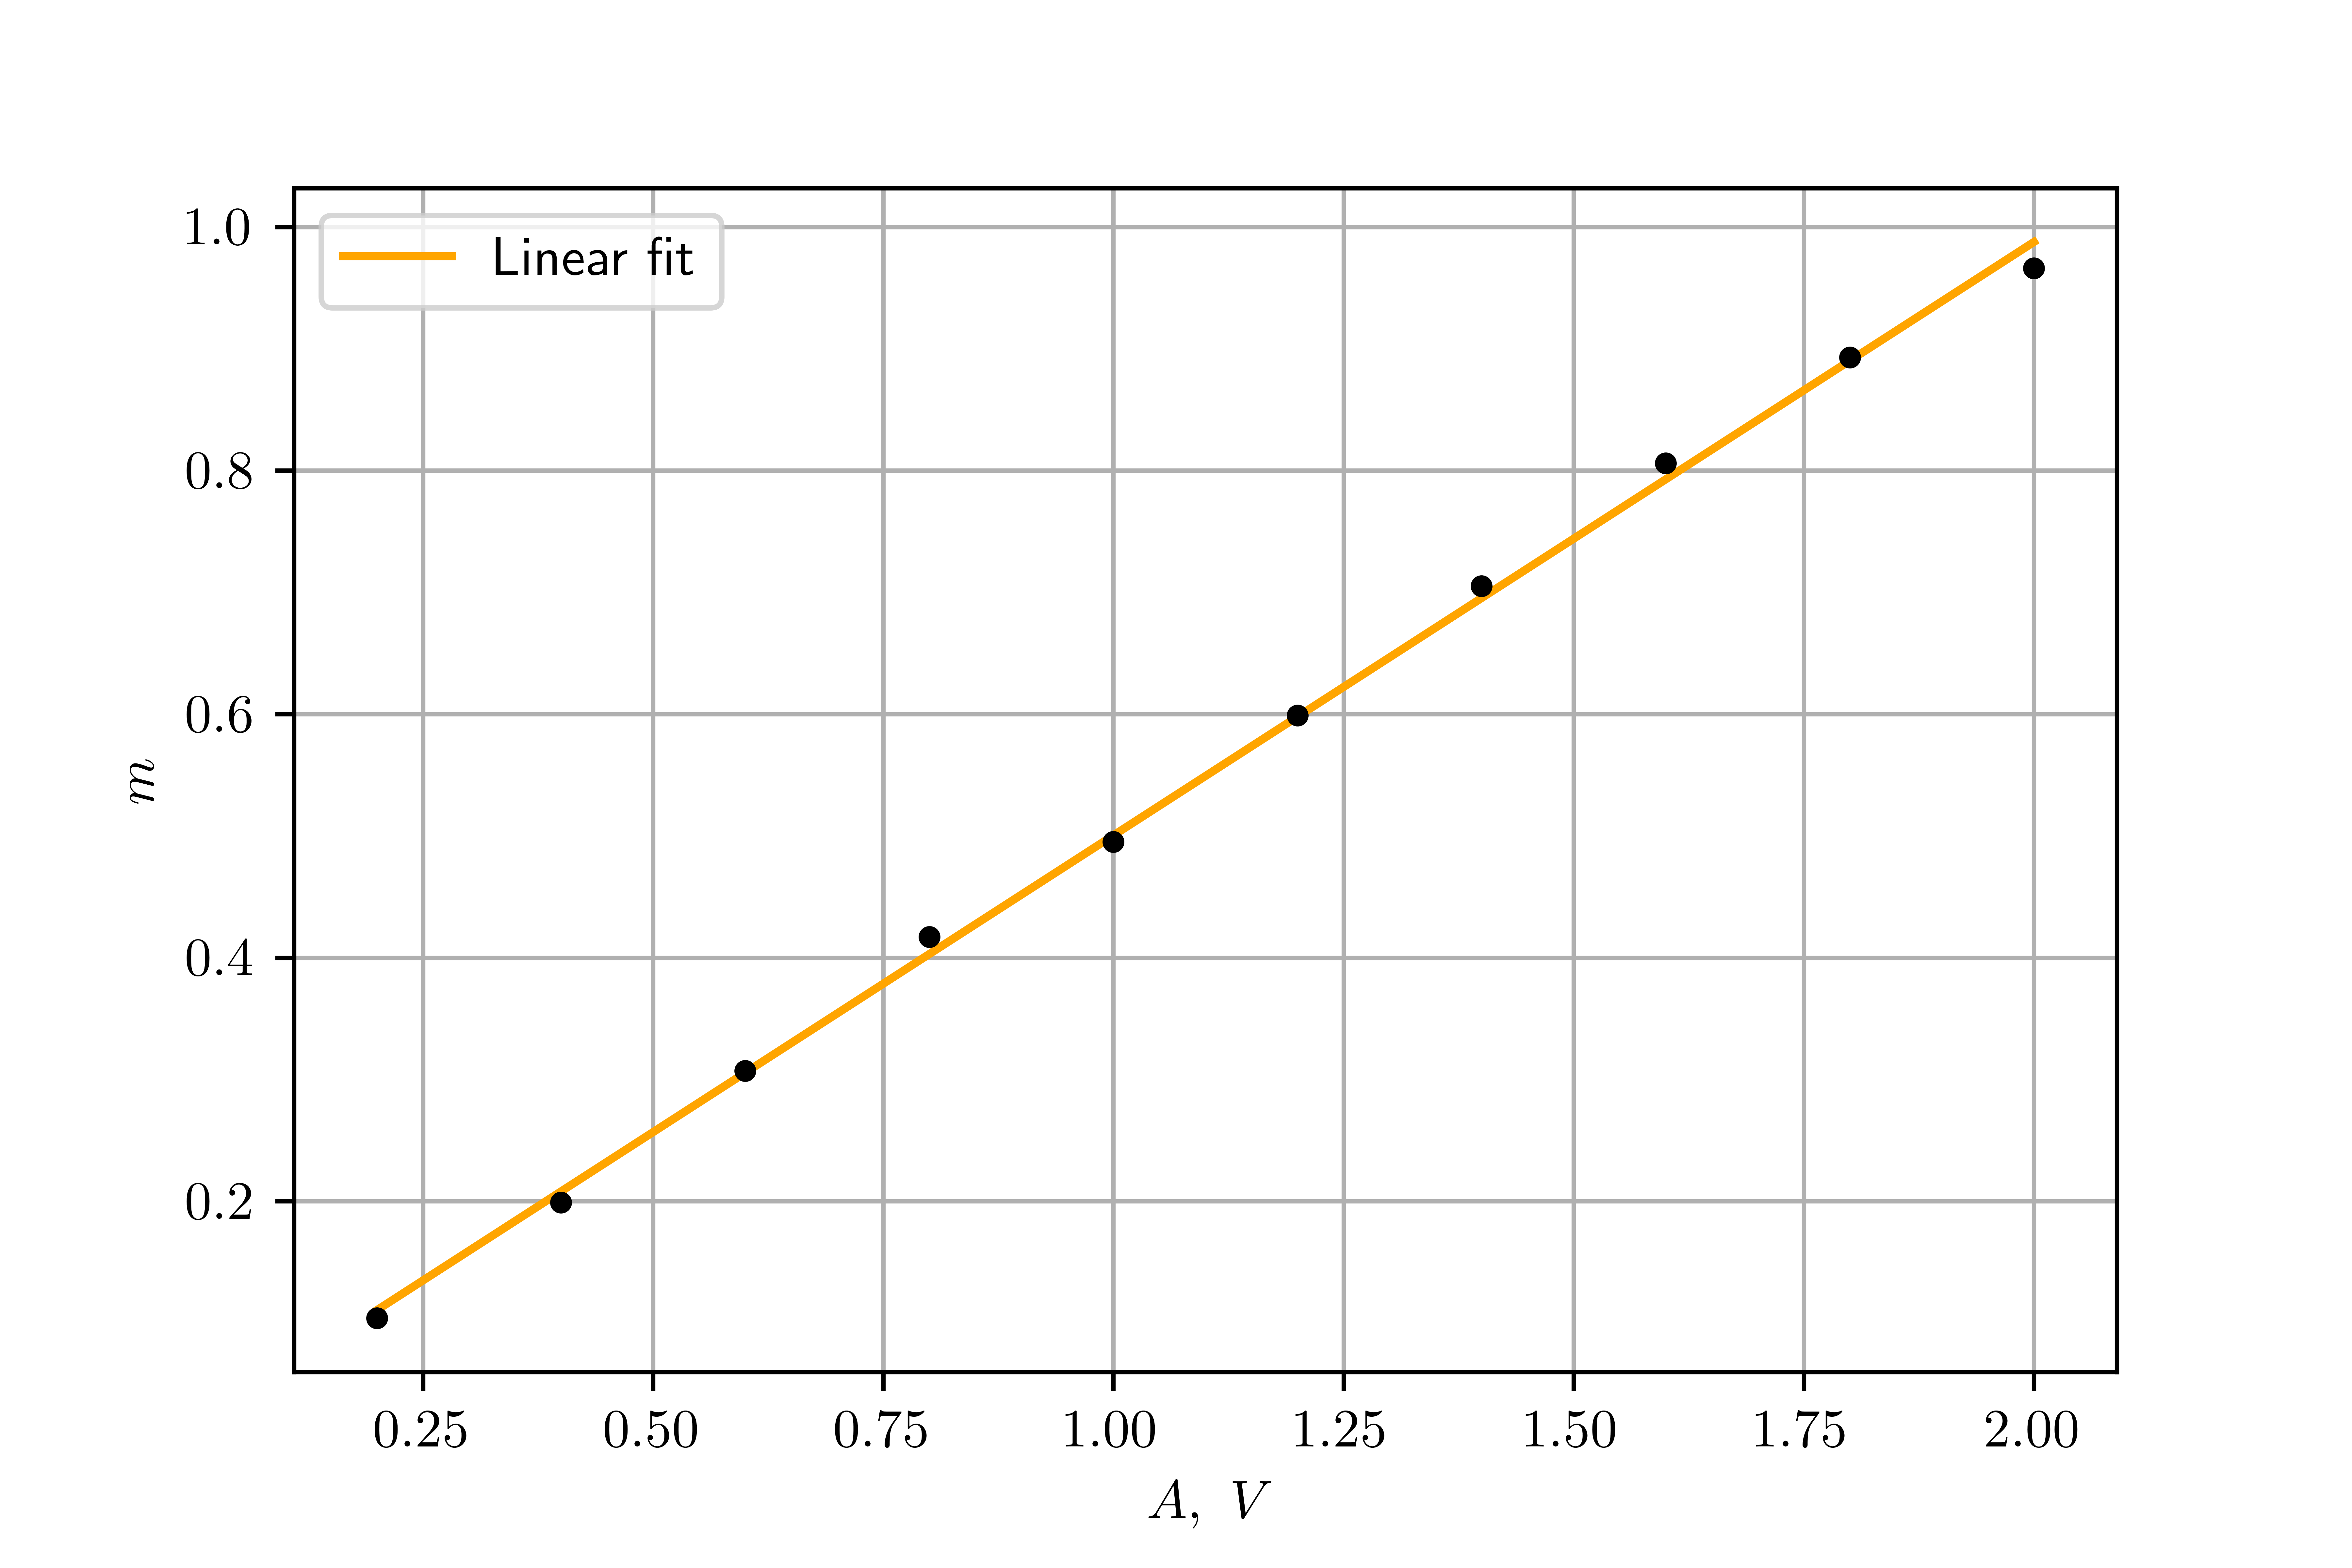
\includegraphics[scale=1]{PIC_13.png}
		\\\textbf{Рис. 13:} График зависимости $m(A)$
	\end{center}
	
	
	\newpage
	
	%Страница 8
	
	\begin{flushleft}
		\footnotesize{Спектральный анализ электрических сигналов} \hspace{\fill} \footnotesize{8}
		\\[-0.3cm]\noindent\rule{\textwidth}{0.3pt}
	\end{flushleft}
	
	Исследуем, теперь отношение $A_{\text{бок}} / A_{\text{осн}}$ от $m$. $A_{\text{осн}}$ = 0.323 V
	
	\begin{center}
		\begin{tabular}{|c|c|c|c|}
			\hline
			$A_{\text{бок}}$, V & $A_{\text{бок}} / A_{\text{осн}}$ & $A$, V & $m$
			\\\hline
			0.0016 & 0.048 & 0.2 & 0.104
			\\\hline
			0.0032 & 0.097 & 0.4 & 0.199
			\\\hline
			0.0048 & 0.149 & 0.6 & 0.307
			\\\hline
			0.0064 & 0.197 & 0.8 & 0.417
			\\\hline
			0.0078 & 0.246 & 1.0 & 0.495
			\\\hline
			0.0094 & 0.289 & 1.2 & 0.599
			\\\hline
			0.0110 & 0.341 & 1.4 & 0.705
			\\\hline
			0.0128 & 0.396 & 1.6 & 0.806
			\\\hline
			0.0142 & 0.440 & 1.8 & 0.893
			\\\hline
			0.0162 & 0.500 & 2.0 & 0.966
			\\\hline
		\end{tabular}
		\\\textbf{Табл. 4:} Зависимость $m(A_{\text{бок}} / A_{\text{осн}})$
	\end{center}

	\begin{center}
		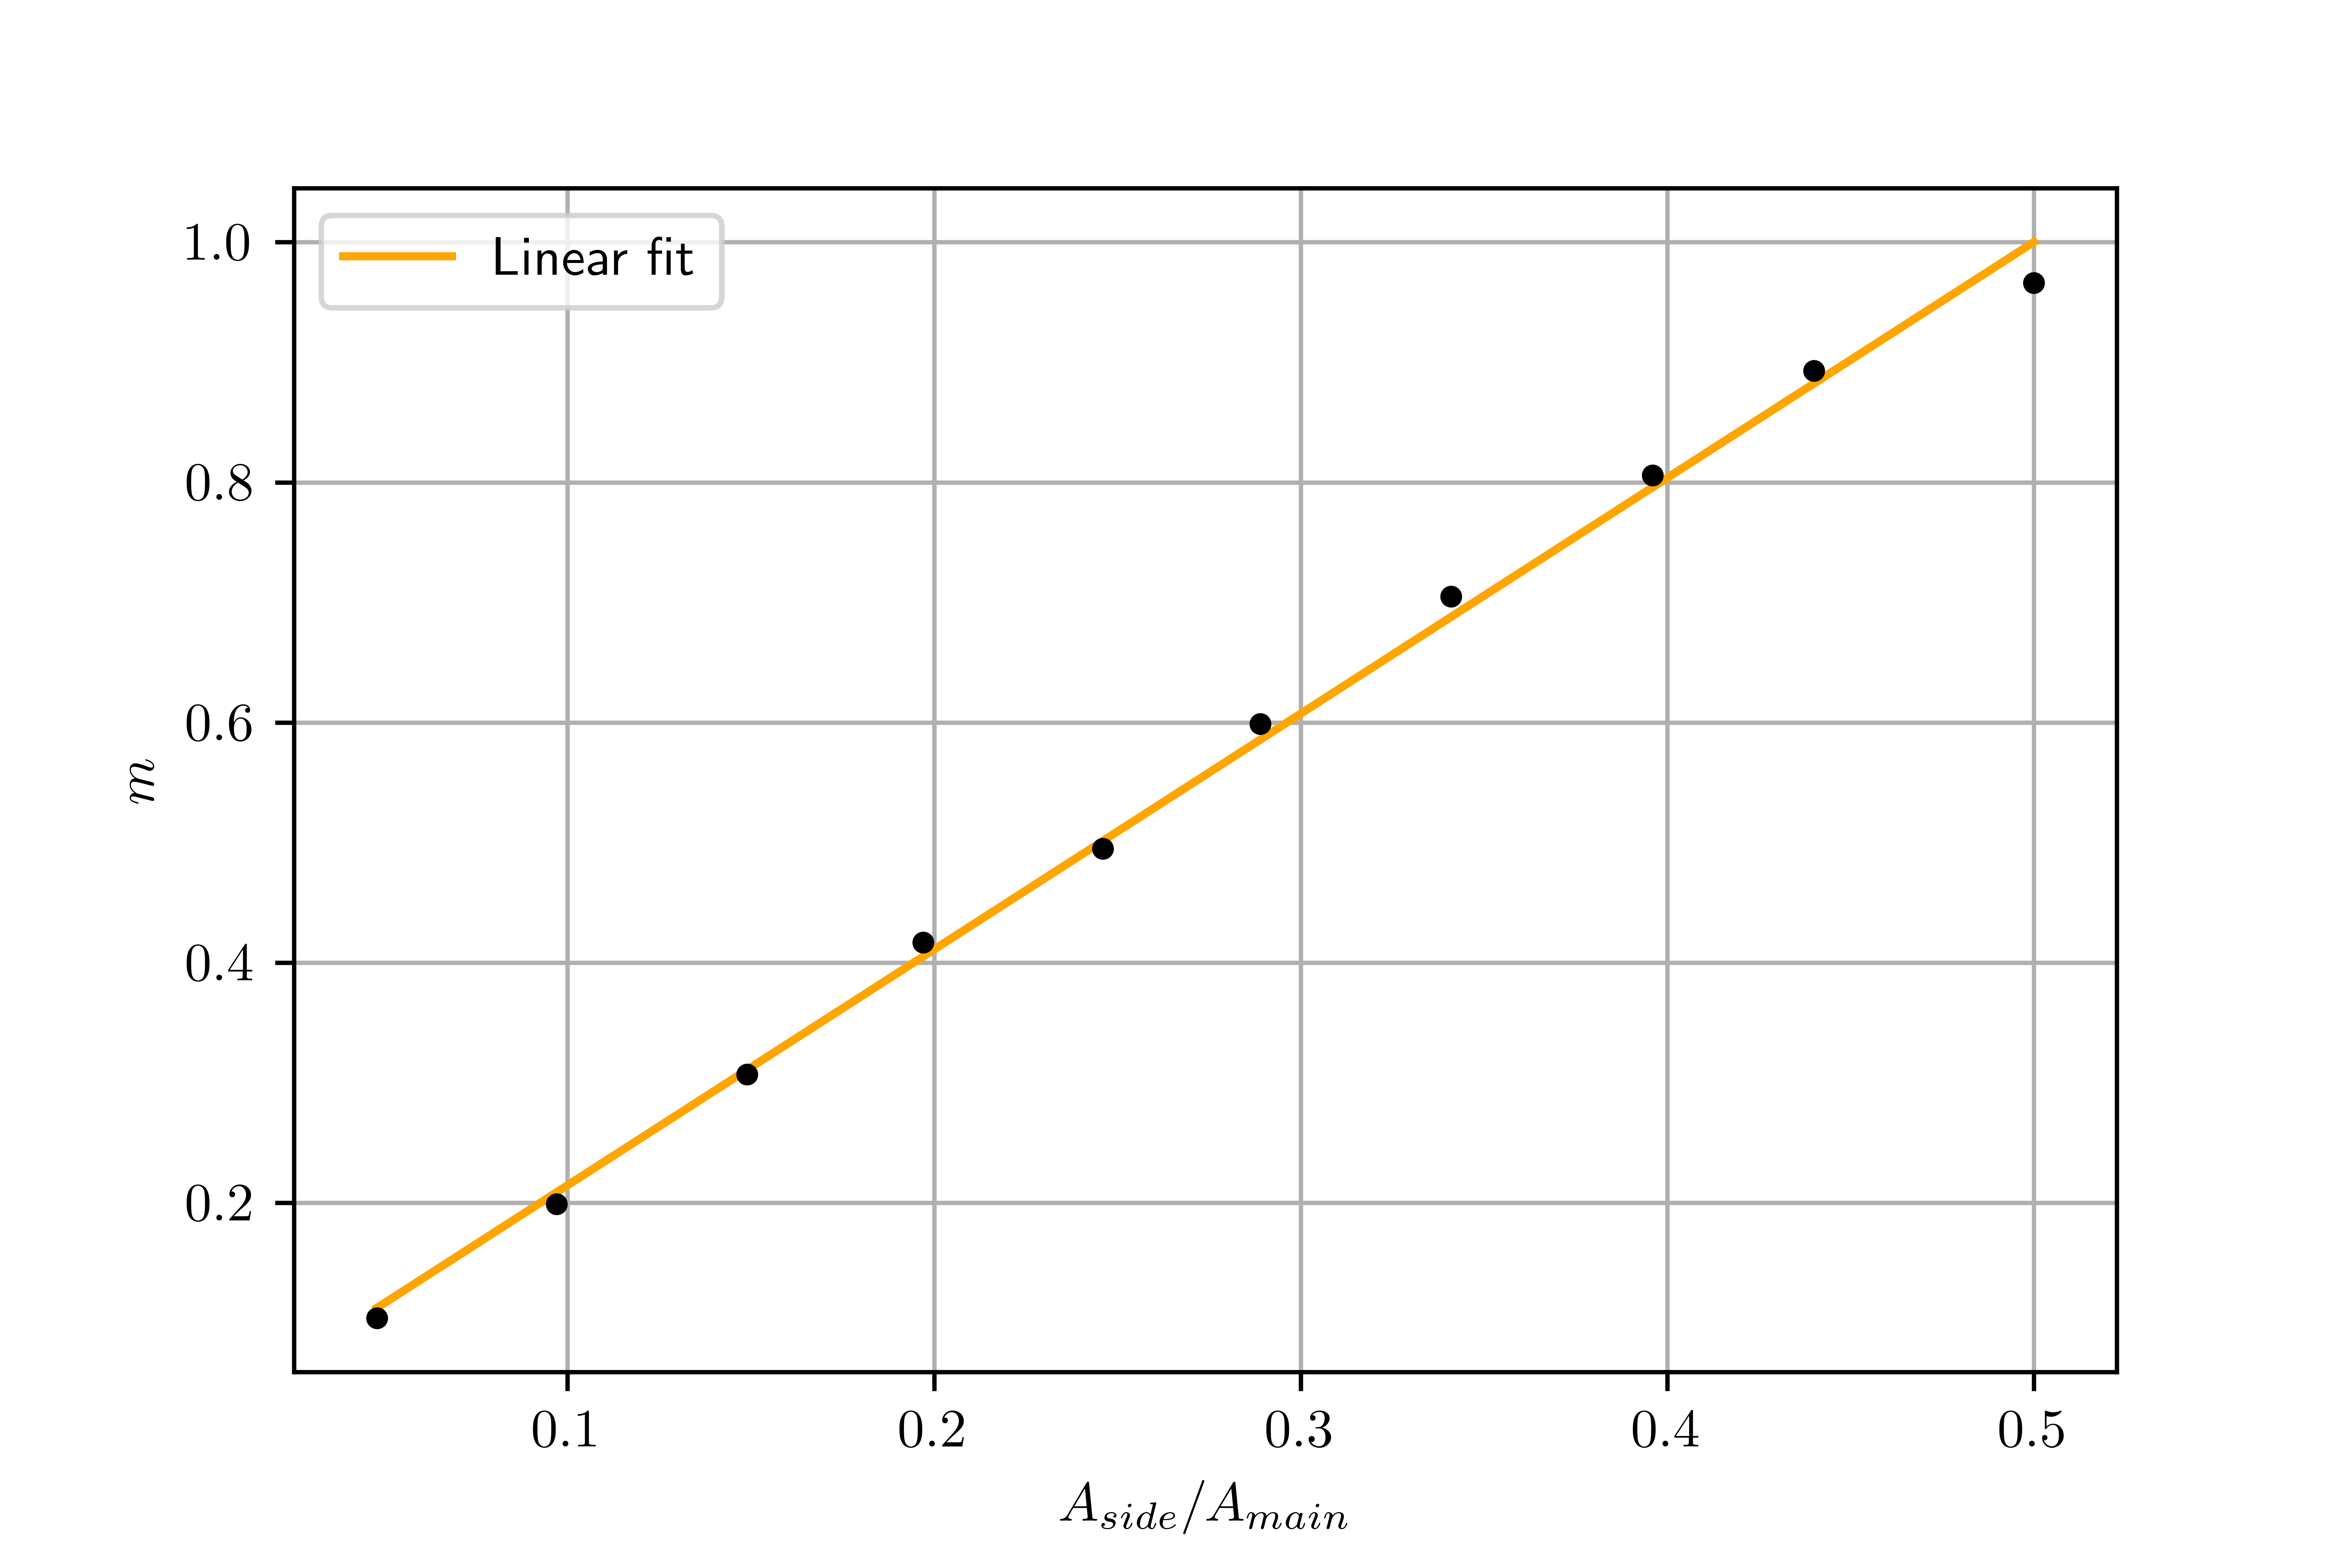
\includegraphics[scale=0.95]{PIC_14.png}
		\\\textbf{Рис. 14:} График зависимости $m(A_{\text{бок}} / A_{\text{осн}})$
	\end{center}
	
	 Из графика видно, что точки хорошо ложатся на прямую. Представив прмяую в виде $m = k(A_{\text{бок}} / A_{\text{осн}}) + b$, получаем методом линейной аппроксимации $k = (1.96 \pm 0.04)$, $b = (0.02 \pm 0.01)$.
	
	\section{Выводы}
	
	Исследования зависимости ширины спектра периодической последовательности прямоугольных импульсов от длительности отдельного импульса в первой части работы полностью совпали с теоретическими рассчетами. По наклону графика из этой части получилось убедиться в соотношении неопределенностей.
	
	Исследования зависимости расстояния между ближайшими спектральными компонентами от частоты повторения цугов дали аналогичные резкльтаты.
	
	В последней части коэффициенты, получаемые в результате исследования зависимости отношения амплитуд спектральных линий синусоидального сигнала, модулированного низкочастотными гармоническими колебаниями, от коэффициента модуляции полностью совпали с теоретически рассчитаными.
	
\end{document}